\documentclass[10pt,letterpaper]{article}
\usepackage[utf8]{inputenc}
\usepackage{amsmath}
\usepackage{amsfonts}
\usepackage{amssymb}
\usepackage{graphicx}
\graphicspath{{./}}
\usepackage[margin=1in]{geometry}
\author{Patrick Duensing}
\title{Steady Hand Project}
\begin{document}
\section{Introduction}
	In this project each person in PHYS213 recorded how steady they could hold their hands using a motion capture device and a green laser. Data was collected from two distances then analyzed using a series of linux commands and programs.
\section{Equipment}
\begin{itemize}
\item MotionLogger
\item Green Laser
\item Linux desktop environment
\end{itemize}
\section{Procedure}
	First a series of data was collected using the MotionLogger device and a green laser. Each student took their turn at a short distance then a long distance. The first step was to get into position at the set point. For the short distance, this was behind the second set of tables in the classroom. For the second set the student was standing behind the last set of desks. After getting into position, the student would aim the laser in the specified area on the whiteboard which had previously been drawn. After doing this they would turn on the laser and try to keep it as steady as possible for just over 10 seconds. After recording the data, Dr. Clark distributed the data via the class website to all the students to analyze using various linux programs.
\section{Results}
	The results show that the standard deviation ranged significantly for the group. The quantatative results of the experiment can be seen in tables \ref{tab:1secshort}, \ref{tab:10secshort}, \ref{tab:1seclong}, and \ref{tab:10seclong}. Further information about the distribution of points can be seen in the histogram in figure \ref{fig:hist}.
\begin{table}[h]
\begin{tabular}{c c c c c c}
Filename & AverageX & AverageY & stddevX & stddevY & TotalDev \\
data-201745135431.txt & 497.375 & 577.75 & 3.29535658162 & 12.0778723292 & 12.51936000762 \\
data-20174513521.txt & 495.666666667 & 587.333333333 & 7.93025150225 & 10.4376455412 & 13.10852140146 \\
data-201745135328.txt & 491.375 & 572.4375 & 4.3928208477 & 12.3779983741 & 13.1343716541 \\
data-201745135111.txt & 498.1875 & 589.8125 & 10.0869268734 & 13.0334605439 & 16.4808127074 \\
data-201745135246.txt & 492.25 & 563.0 & 14.0934381895 & 27.8758407945 & 31.2359968626 \\
\end{tabular}
\caption{\label{tab:1secshort}A table of the results from the short distance experiment for the first second}
\end{table}
\begin{table}[h]
\begin{tabular}{c c c c c c}
Filename & AverageX & AverageY & stddevX & stddevY & TotalDev \\
data-201745135944.txt & 506.125 & 574.1875 & 5.17656981021 & 12.7351322628 & 13.74701672185 \\
data-20174513577.txt & 472.666666667 & 579.5 & 15.3188337241 & 25.7811300502 & 29.9888868304 \\
data-201745135616.txt & 474.8125 & 589.375 & 12.3286695856 & 28.6626390097 & 31.2016500966 \\
data-201745135851.txt & 491.625 & 596.9375 & 23.3475774975 & 30.1635515772 & 38.1437965959 \\
data-20174513581.txt & 524.9375 & 598.5625 & 21.5789792101 & 32.3606990615 & 38.8955934200 \\
\end{tabular}
\caption{\label{tab:10secshort}A table of the results from the long distance experiment for the first second}
\end{table}
\begin{table}[h]
\begin{tabular}{c c c c c c}
Filename & AverageX & AverageY & stddevX & stddevY & TotalDev \\
data-201745135431.txt & 499.927631579 & 572.401315789 & 6.87802753787 & 12.5365307614 & 12.51936000762 \\
data-20174513521.txt & 492.327160494 & 577.561728395 & 8.04469017958 & 18.409502162 & 13.10852140146 \\
data-201745135328.txt & 479.344155844 & 580.733766234 & 25.5599955974 & 32.8824731682 & 13.1343716541 \\
data-201745135111.txt & 493.39375 & 576.40625 & 8.61455663035 & 15.6151156236 & 16.4808127074 \\
data-201745135246.txt & 485.550632911 & 574.772151899 & 14.8989412029 & 23.4139682247 & 31.2359968626 \\
\end{tabular}
\caption{\label{tab:1seclong}A table of the results from the short distance experiment for the first ten seconds}
\end{table}
\begin{table}[h]
\begin{tabular}{cccccc}
Filename & AverageX & AverageY & stddevX & stddevY & TotalDev \\
data-201745135944.txt & 502.820512821 & 541.25 & 9.91760102008 & 21.9667216255 & 13.74701672185 \\
data-20174513577.txt & 489.301282051 & 586.121794872 & 17.2863032603 & 27.9291899845 & 29.9888868304 \\
data-201745135616.txt & 487.681818182 & 590.5 & 19.0295240693 & 34.7532115679 & 31.2016500966 \\
data-201745135851.txt & 494.953947368 & 586.526315789 & 20.66082258 & 27.8980633568 & 38.1437965959 \\
data-20174513581.txt & 475.126582278 & 593.981012658 & 41.6203051372 & 55.0810359884 & 38.8955934200 \\
\end{tabular}
\caption{\label{tab:10seclong}A table of the results from the long distance experiment for the ten seconds}
\end{table}
\begin{figure}[h]
\centering
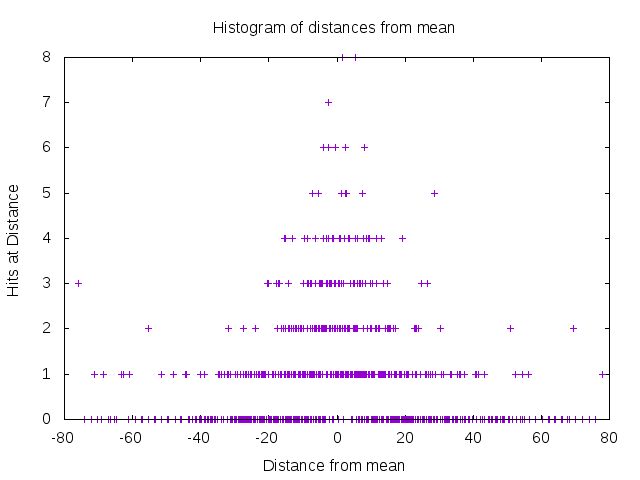
\includegraphics[width=0.5\textwidth]{histogram}
\caption{\label{fig:hist}Graph of the distances of all points within ten seconds from the mean}
\end{figure}
\end{document}
